\subsection{Levantamento das características dos edifícios de escritório de Vitória}
As edificações de escritório de Vitória selecionadas após a definição do recorte territorial, apresentam características que foram complementadas aos atributos observados em edificações comerciais brasileiras, como suporte as informações não encontradas in loco. As características com maior frequência de ocorrência no levantamento realizado são apresentadas na Tabela \ref{tab:tabela4}. Todavia, a amostra coletada abrange edifícios iniciados em 2003 e concluídos até o fim do primeiro trimestre de 2018, data do início do levantamento. Este fato inviabiliza aplicar a última revisão do Plano à amostra.\newline \vspace*{0.3cm}
Foram considerados para o levantamento atributos como gabarito, número de pavimentos-tipo, número de salas por pavimento-tipo, dimensão e forma, altura dos pavimentos-tipo. Não foram consideradas as dimensões dos lotes onde as edificações da amostra estacam implantadas, já que este atributo não foi pertinente ao objetivo do trabalho. Estes parâmetros foram reunidos em consulta ao material técnico disponibilizado pelas construtoras, visitas a campo e complementação de dados utilizando a ferramenta computacional \textit{Google Street View}.\newline \vspace*{0.3cm}
Os trabalhos de \textcite{Lamberts2006,AmericanSocietyofHeatingRefrigeratingandAir-ConditioningEngineers-ASHRAE2010,Bernabe2012,Ramos2013,Didone2014,Didone2014a,ConselhoBrasileirodeConstrucaoSustentavel-CBCS2015,Fonseca2016,Werneck2017,InstitutoNacionaldeMetrologiaNormalizacaoeQualidadeIndustrial-INMETRO2018}, foram utilizados como principais fontes de informação para a análise de envoltória e sistema de iluminação e condicionamento de ar.%\vspace{-0.25cm}
    \begin{table}[H]
        \centering
        \small
        \caption{Características observadas em campo e em pesquisas anteriores.}
        \begin{tabular*}{\columnwidth}{@{\extracolsep{\fill}}lll}
        \hline
        \textbf{Parâmetro}                                             & \textbf{Descrição}                                                                    & \textbf{Referências} \\ \hline
        Gabarito                                                       & 24 a 60 m (8 a 19 pav.)                                                               & \makecell[l]{Levantamento \textit{in loco} e referências\\ (BERNABÉ, 2012; CBCS, 2015; \\FONSECA et al., 2016; LAMBERTS; \\GHISI; RAMOS, 2006; RAMOS \\et al., 2013).} \\ \hline
        Altura do pavimento                                            & 3 m                                                                                   & Levantamento \textit{in loco}.                                                                                                                                         \\ \hline
        Planta-baixa (forma)                                           & Retangular                                                                            & \makecell[l]{Levantamento \textit{in loco} e referências\\ (FONSECA et al., 2016; INMETRO,\\ 2018).}                                                                   \\ \hline
        \makecell[l]{Dimensão das salas\\ por pav.-tipo}               & 40 m²                                                                                 & \makecell[l]{Foi fixado a área das salas \\(zonas térmicas) de acordo com a \\média de ofertas de salas observadas\\ em levantamento \textit{in loco}.}                  \\ \hline
        \multicolumn{3}{c}{Continua}\\\hline
    \end{tabular*}
    \label{tab:tabela4}
    \end{table}\pagebreak
    \begin{table}[H]
        \centering
        \small
        \begin{tabular*}{\columnwidth}{@{\extracolsep{\fill}}lll}
        \hline
        \multicolumn{3}{c}{Conclusão}\\\hline
        \makecell[l]{Componentes da\\ parede}                          & \makecell[l]{Bloco cerâmico,\\ 8 furos; \\14x19x29 cm; \\argamassa de\\ assentamento} & Levantamento \textit{in loco}.                                                                                                                                         \\ \hline
        Proteção solar                                                 & Sem proteção                                                                          & \makecell[l]{Levantamento \textit{in loco} e referências\\ (FONSECA et al., 2016; WERNECK \\et al., 2017).}                                                            \\ \hline
        Cobertura                                                      & \makecell[l]{Laje impermeabilizada\\ com 20 cm de\\ espessura}                        & \makecell[l]{Levantamento \textit{in loco} e referências \\(CB3E; ABIVIDRO, 2015).}                                                                                    \\ \hline
        Vidros                                                         & \makecell[l]{Laminado; Reflexivo;\\ 8 mm; Verde}                                      & \makecell[l]{(FONSECA et al., 2016; \\INMETRO, 2018).}                                                                                                                   \\ \hline
        PAF\textsubscript{T}                                           & 30\%; 50\%; 80\%                                                                      & \makecell[l]{Levantamento \textit{in loco}\\ e referências.}                                                                                                             \\ \hline
        \makecell[l]{Orientação solar da \\fachada principal}          & Sul                                                                                   & \makecell[l]{Levantamento \textit{in loco}\\ e referências.}                                                                                                             \\ \hline
        \makecell[l]{Densidade de Carga de\\ Iluminação Limite – DCIL} & 14,1 W/m²                                                                             & \makecell[l]{Consulta pública do RTQ-C \\(INMETRO, 2018).}                                                                                                               \\ \hline
        \makecell[l]{Densidade de Carga de\\ Equipamentos – DCE}       & 9,7 W/m²                                                                              & \makecell[l]{Consulta pública do RTQ-C \\(INMETRO, 2018).}                                                                                                               \\ \hline
        \makecell[l]{Absortância/transmitância \\das paredes}          & \makecell[l]{0,59 (cor \\camurça)/3,75}                                               & \makecell[l]{Valores consultados na \\NBR 15220-2 e referências \\(ABNT, 2003; FONSECA et \\al., 2016; INMETRO, 2018).}                                                                     \\ \hline
        \makecell[l]{Absortância/transmitância \\das coberturas}       & \makecell[l]{0,65 (concreto \\aparente)/2,06}                                         & \makecell[l]{Valores consultados na \\NBR 15220-2 e referências \\(ABNT, 2003; FONSECA et \\al., 2016; INMETRO, 2018).}                                                 \\ \hline
        \end{tabular*}
        \begin{flushleft}
            \par \small Fonte: autor (2019).
        \end{flushleft}
    \end{table}\vspace*{-0.3cm}

\noindent As informações coletadas nos estudos e em levantamento formam a base conceitual para determinar os aspectos arquitetônicos relevantes para compor os modelos genéricos e, posteriormente, determinar os parâmetros de otimização e do consumo energético padrão aproximado para um edifício de escritório. Além disso, a quantidade de simulações necessárias para determinar o consumo de energia dos modelos genéricos é identificada por meio da organização dos dados coletados em campo e, assim, a resultante do número de variáveis.

\subsubsection{Consumo de energia elétrica das edificações}
\noindent O consumo de energia elétrica em edificações de escritório no Brasil é determinado principalmente por sua tipologia. As configurações predominantes no Brasil compreendem, em sua maioria, pequenas edificações, abaixo de 8 pavimentos, a edifícios grandes, acima de 15 pavimentos \cite{Carlo2008,Ramos2013,ConselhoBrasileirodeConstrucaoSustentavel-CBCS2015,Fonseca2016}.\newline
\noindent Correlacionado às tipologias arquitetônicas, os dados de consumo de energia, expressos em Intensidade de Uso de Energia – IUE, kWh/m²/ano, foram necessários para validação das simulações iniciais quanto ao consumo de energia esperado dos modelos. Visto que a calibração dos modelos genéricos não foi possível, pois eles não dispunham de memorial de massa como ferramenta de comparação ao consumo simulado computacionalmente, foram adotados como método de comparação os valores médios registrados no Relatório Final do CBCS (2015), como mostra o Histograma no Gráfico 5. Foi relacionado o consumo de energia das edificações levantadas à frequência de ocorrência da quantidade de pavimentos de edificações comerciais brasileiras e suas respectivas áreas comuns.\newline

    \begin{graph}
        \par \small Gráfico 5 - Consumo energético em edificações de escritório brasileiras.
        \begin{minipage}[ht]{1\textwidth}\centering
            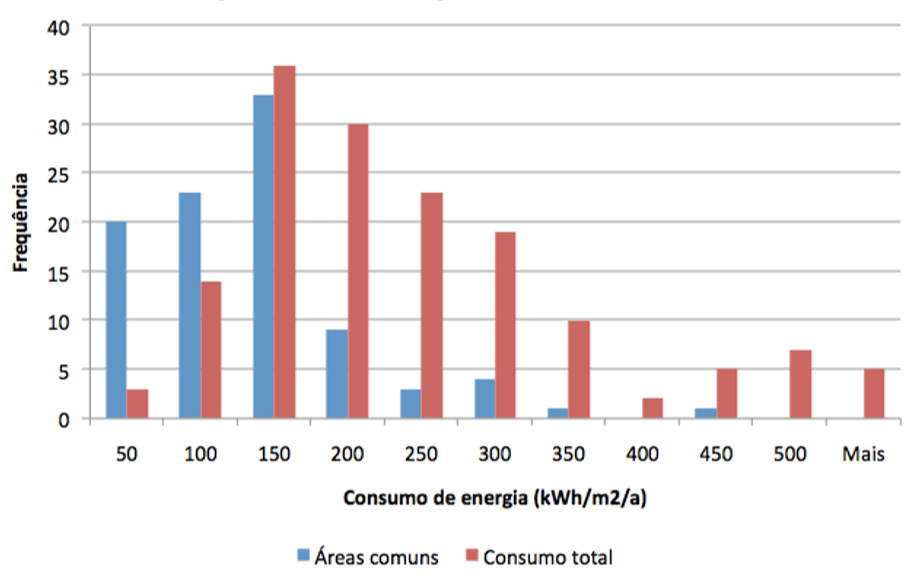
\includegraphics[width=1.0\textwidth]{figures/fig9_consumo-total-das-edificacoes-levantadas_cbcs_2015.png}            
        \end{minipage}
        \begin{flushleft}
            \par \small Fonte: adaptado de CBCS (2015).
        \end{flushleft}
    \end{graph}

\noindent Logo, os dados de IUE adotados para a comparação e avaliação inicial do consumo energético dos modelos foram baseados nos valores máximo e mínimo estabelecidos pelo CBCS (2015). A média entre o consumo em áreas comuns e total relacionado à frequência de quantidade de pavimentos define a quantidade total de consumo de energia para cada tipologia.\vspace*{0.3cm} \newline
Os autores do Relatório atribuem 133 kWh/m²/ano aos edifícios de pequeno porte, e 268 kWh/m²/ano às edificações de grande porte. Vale ressaltar que os dados de consumo energético, assim como a média apontada no Relatório, de 191 kWh/m²/ano, desprezam as distorções causadas por edificações com particularidades de consumo como datacenters ou erros de cálculo de área útil.\vspace*{0.3cm} \newline
Ao estabelecer as Intensidades de Uso de Energia equivalentes a cada modelo, assim como os padrões de uso e ocupação, pode-se estimar o consumo de energia durante determinado período.

\subsubsection{Padrões de uso e ocupação em edifícios de escritório}
Os padrões de uso e ocupação da edificação foram baseados em normas, regulamentos, relatórios técnicos e referências acadêmicas que consideraram os níveis de atividades desenvolvidas nos ambientes, tratadas neste trabalho como zonas térmicas, como apresentado na Tabela \ref{tab:tabela5}.\vspace*{0.3cm} \newline
Como o intuito do trabalho foi criar modelos genéricos que representassem minimamente o cenário encontrado na cidade de Vitória, as características de uso e ocupação escolhidas foram integradas como forma de aproximar as tipologias ao cenário observado. Dentre elas, pode-se citar:
\begin{itemize}
    \item O nível metabólico apresentado em atividades de escritório;
    \item O horário de funcionamento dos escritórios, determinando os intervalos de tempo de ocupação total e parcial, onde, respectivamente, a capacidade máxima e parcial de ocupação das zonas térmicas é atingida;
    \item A densidade de pessoas por metro quadrado para cada zona térmica;
    \item A temperatura de conforto em cada zona térmica, de acordo com as normas de conforto térmico consultadas; e
    \item A umidade relativa do ar nos ambientes de escritório.
\end{itemize}

\noindent A obtenção dos dados acerca da atividade desempenhada nas edificações de escritório, além do horário de funcionamento e densidade de ocupação serão utilizados para estimar o consumo de energia elétrica do espaço utilizado por meio de simulação computacional.
\begin{table}[H]
    \centering
    \small
    \caption{Padrões de uso e ocupação}
    \begin{tabular*}{\columnwidth}{@{\extracolsep{\fill}}llll}
        \hline
        \textbf{Parâmetro}                                & \multicolumn{2}{c}{\textbf{Descrição}}                                                                                             & \textbf{Referências} \\ \hline
        \multirow{2}{*}{Atividades}                       & \makecell[l]{Escritório:\vspace*{0,2cm}\\Fator metabólico:\vspace*{0,2cm}} & \makecell[l]{Leve\vspace*{0,2cm}\\0,9 met}                  & \makecell[l]{As salas de escritório da cidade\\
                                                                                                                                                                                        são utilizadas, em sua maioria,\\ para 
                                                                                                                                                                                        atividades especializadas de\\ âmbito 
                                                                                                                                                                                        jurídico, relacionadas à \\construção 
                                                                                                                                                                                        civil, a saúde e atividades\\ financeiras.} \\ \hline
        \multicolumn{4}{c}{Continua}\\\hline
    \end{tabular*}
    \label{tab:tabela5}
\end{table}\pagebreak

\begin{table}[H]
        \centering
        \small
        \begin{tabular*}{\columnwidth}{@{\extracolsep{\fill}}llll}
        \hline
        \multicolumn{4}{c}{Conclusão}\\\hline
        \multirow{2}{*}{Horário de funcionamento}                          & \makecell[l]{Ocupação\\ total:\vspace*{0,2cm}\\Ocupação \\parcial (50\%):\vspace*{0,6cm}}  & \makecell[l]{8h às 12h; \\13h às 18h \vspace*{0,6cm}\\12h às 13h} & \makecell[l]{Segundo normas e pes-\\quisas
                                                                                                                                                                                                                                                sobre o horário de\\ funcionamento de 
                                                                                                                                                                                                                                                escri-\\tórios, o início da ocupa-\\ção se 
                                                                                                                                                                                                                                                dá às 6h e pode se\\ estender até às 24h.\\ 
                                                                                                                                                                                                                                                Entretanto, visando a\\ aproximação às 
                                                                                                                                                                                                                                                condi-\\ções praticadas no\\ mercado brasileiro,\\ 
                                                                                                                                                                                                                                                adota-se a redução\\ de ocupação durante\\ o 
                                                                                                                                                                                                                                                horário de almoço, \\denominada ocupação\\ parcial.}  \\ \hline
        Densidade de ocupação                             & \multicolumn{2}{c}{0,14 pessoas/m²} & \makecell[l]{(CONSELHO BRASILEIRO\\ DE CONSTRUÇÃO 
                                                                                                  SUS-\\TENTÁVEL - CBCS, 2015;\\ LAMBERTS; 
                                                                                                  GHISI;\\ RAMOS, 2006; MORAES;\\ PEREIRA, 2014).} \\ \hline
        Temperatura de controle                           & \multicolumn{2}{c}{24°C}            & \makecell[l]{Temperatura limite de\\ acionamento
                                                                                                  do sistema de\\ condicionamento de\\ ar (ASHRAE, 
                                                                                                  2010, 2017a;\\ INMETRO, 2010a).} \\ \hline
        \makecell[l]{Nível de iluminância\\ de referência}& \multicolumn{2}{c}{500 lux}         & \makecell[l]{Iluminância mínima (entor-\\no de 
                                                                                                  trabalho) para ativi-\\dades visuais 
                                                                                                  (ASHRAE,\\ 2010; ABNT, 2013).} \\ \hline
        \makecell[l]{Umidade Relativa\\ Interna}          & \multicolumn{2}{c}{40\%-60\%}       & \makecell[l]{Faixa recomentada pela\\
                                                                                                  ASHRAE 55 (2017a).}\\ \hline
    \end{tabular*}
    \begin{flushleft}
        \par \small Fonte: autor (2019).
    \end{flushleft}
\end{table}
